%%%%%%%%%%%%%%%%%%%%%%%%%%%%%% -*- Mode: Latex -*- %%%%%%%%%%%%%%%%%%%%%%%%%%%%
%% 00slides.tex 
%% Author          : Yaakov Oshman
%% Created On      : Thu Apr 15 22:28:37 2004
%% Last Modified By: Yaakov Oshman
%% Last Modified On: Thu Feb 11 16:39:30 2010
%% Update Count    : 412
%% Status          : Unknown, Use with caution!
%%%%%%%%%%%%%%%%%%%%%%%%%%%%%%%%%%%%%%%%%%%%%%%%%%%%%%%%%%%%%%%%%%%%%%%%%%%%%%%
        
%% PROCESSING THE LATEX FILE (use both input and output file names!):
%%    1. latex file.tex
%%    2. dvips -ta4 -Ppdf file.dvi -o file.ps  (a4 page size)
%%    3. ps2pdf -r1200 file.ps file.pdf (1200 resolution)

       
\documentclass[mathserif]{beamer}
%%\documentclass[gray,handout,mathserif]{beamer}

%%\documentclass[mathserif,allowframebreaks,shrink]{beamer}
%% frame options:
%%  
%% [squeeze] for squeezing vertical space
%% [shrink] for shrinking the content to fit in a single slide
%% \frame[plain]{\frametitle{}...} for plane frame style
%% [allowframebreaks] automatic splitting of frame if content does not
%% fit in a single slide


%\usetheme{split}    % takes more vertical space!!
%\usetheme{Berkeley} % vertical side navigation bar
%\usetheme{Malmoe}
%\usetheme{shadow}
%\usetheme{PaloAlto}  %  side nav bar
%\usetheme{Copenhagen}  %  top nav bar
%\usetheme{Madrid}  %  no nav bar
\usetheme{Boadilla}  % nice and clean, no nav bar, max space!
%\usetheme{montpellier}  %  top tree
%\usetheme{Singapore}  %  top (sort of tree)
%\usetheme{pittsburgh}   % no nav bar, clean, takes more space than Boadilla...
%\usetheme{szeged}

\setbeamertemplate{navigation symbols}{}  %no nav symbols at bottom of PDF
%% or
%% \usenavigationsymbolstemplate{}
%%



\usepackage{eulervm}
%%\usepackage[small]{eulervm}

%%\beamertemplateballitem    %% fancy bulletts

\usepackage{colordvi}  %% texmf/tex/generic/dvips/colordvi.tex (names
                       %% of all predefined colors)

\usepackage{amsmath}
\usepackage{amssymb}
\usepackage{amsfonts}
\usepackage{amsthm}
\usepackage{bm}
\usepackage{xspace}
\usepackage{latexsym}
\usepackage{mathrsfs}
\usepackage{wasysym}
%\usepackage{arydshln}
\usepackage{eulervm}
\usepackage[T1]{fontenc}
\usepackage{aurical}


\graphicspath{{Figures/}}
\DeclareGraphicsRule{*}{eps}{*}{}
%\DeclareGraphicsExtensions{.eps}

\newcommand{\epspath}{}
%\newcommand{\epspath}{g:/usr1/etc/logos/}
   
\newenvironment{slidelist}{\begin{list}{$\bullet$}%
    {\itemsep -0.5ex \topsep -2ex \partopsep 0ex}}{\end{list}}

\newenvironment{smilebullet}{\begin{list}{{\large \green \smiley}}%
{\itemsep 1ex \partopsep 0ex}}{\end{list}}

\newenvironment{frownbullet}{\begin{list}{{\large \green \frownie}}%
{\itemsep 1ex  \partopsep 0ex}}{\end{list}}

\newcommand{\subheading}[1]{\textbf{\textsf{{\textcolor{blue}{#1}}}}}
\newcommand{\subsubheading}[1]{\textbf{\textsf{\textcolor{red}{#1}}}}


\title[BLOM]{{\bf BLOM}: {\bf B}erkeley {\bf L}ibrary for \\ 
  {\bf O}ptimization {\bf M}odeling}
%
\author[S. Vichik, A. Kelman]{Sergey Vichik
%
  ~and~Anthony Kelman }


\date[March 2012]{March, 2012}

\institute[UC Berkeley]{UC Berkeley\\
  Department of Mechanical Engineering\\
  Berkeley, CA \\[1ex]
  sergv@berkeley.edu, \hspace{1em}
}

%

\renewcommand{\include}{\input}       


         
\begin{document}

%
\begin{frame}
  \titlepage
\end{frame}
%

%\begin{frame} \frametitle{Outline}
%  \tableofcontents
%\end{frame}
%
%\include{abstract}
%%\tableofcontents[current]

\begin{frame}
\frametitle{What is BLOM ?}
\begin{itemize}
\item A language of modeling
dynamical nonlinear systems for optimization problems, especially MPC.
\item Support for the following design phases:
\begin{itemize}
\item Developing the model with an intuitive block diagram.
\item Forward simulation and validation of the model.
\item Automatic export of the optimization problem to a solver. 
\end{itemize}
\item Developed to handle non trivial problems
\begin{itemize}
\item C++ or Matlab code generation.
\item Explicit evaluation of Jacobian and Hessian.
\item Proven with problems of tens of thousands variables.
\end{itemize}
\item Eliminates manual problem coding, eases maintenance and assures that the
  same model used for optimization and for simulation.
\end{itemize}
\end{frame}

\begin{frame}
\frametitle{''Hello World'' example}

\centering 
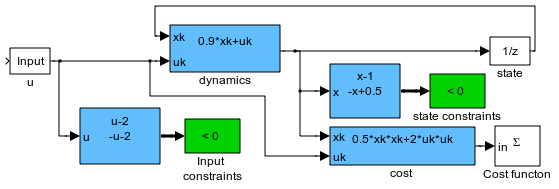
\includegraphics[width = .7\textwidth]{HelloWorld}

\begin {align}
\min_{u_k,x_k}& \sum_k 0.5x_k^2 + 2u_k^2 \notag \\
s.t.:&  -2 \leq u_k \leq 2 \ ; 0.5 \leq x_k \leq 1;x_{k+1}=0.9x_k+u_k
\end{align}

\begin{itemize}
\item Block library for Simulink:
\begin{itemize}
\item The functional block is a function of the form $\frac{f(x)}{g(x)}$,
  where $f$ or $g$ are:  $f,g=\sum_i \prod_j
v_{i,j}(x_i)$.  $v(x_i)$ can be $x^p$ for any $p \in \mathbb R$, $\exp(x)$ or
$\log(x)$. 
\item Constraint
\item State
\item Cost 
\item Input/External variable modifiers
\end{itemize}
\end{itemize}
\end{frame}
             
\end{document}

\endinput

